\documentclass{standalone}
\usepackage{tikz}
\usetikzlibrary{patterns, positioning}


\begin{document}
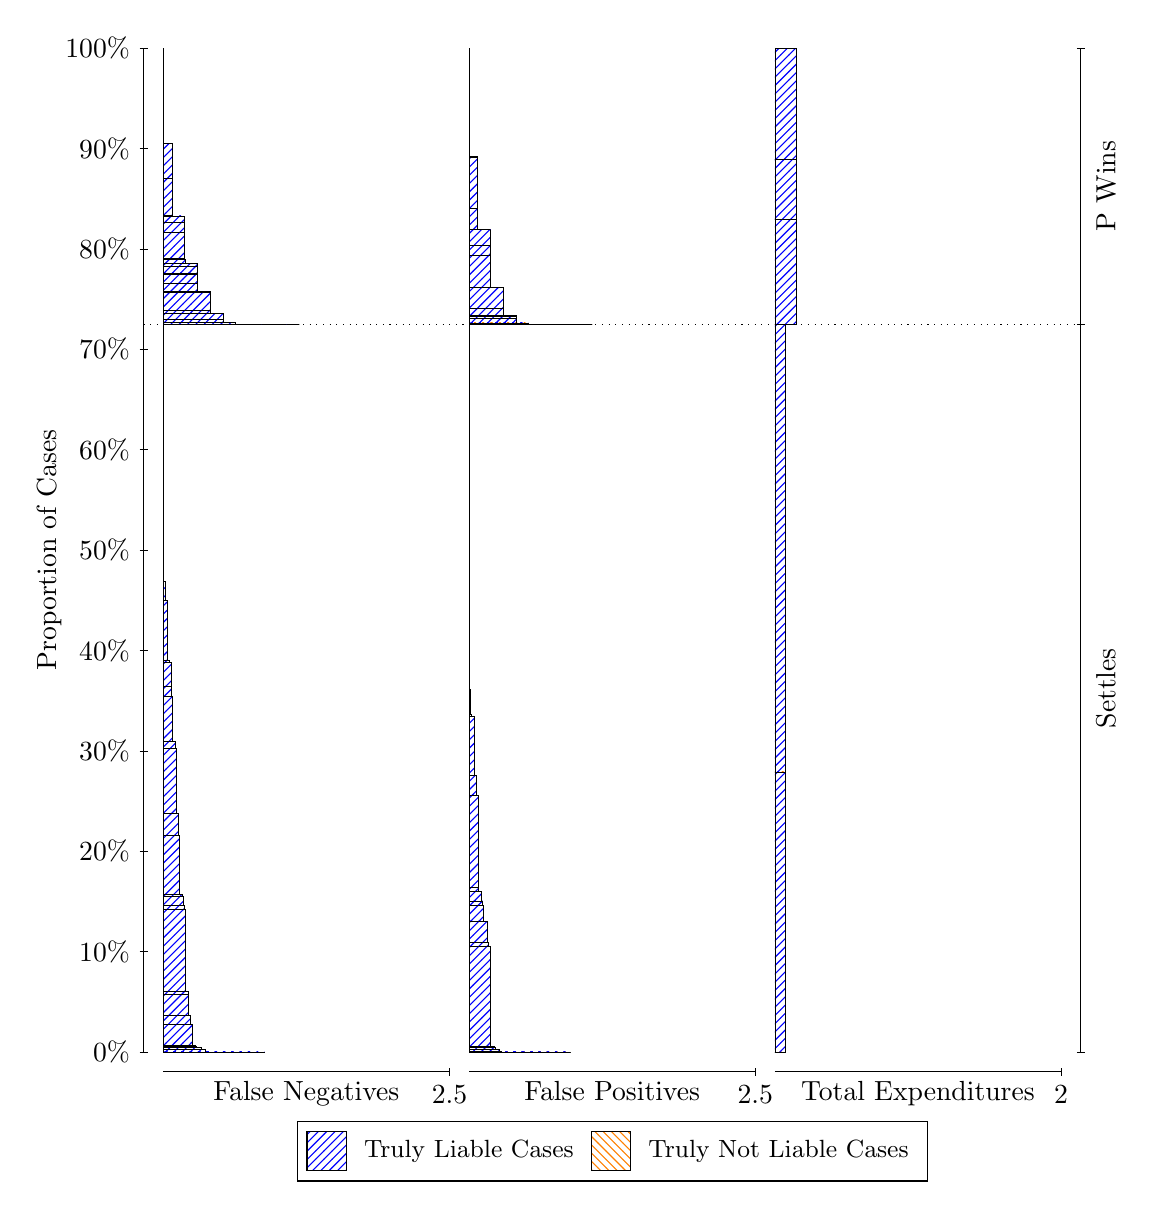
\begin{tikzpicture}
\draw[black, very thin] (1.5,1.75) -- (1.5,14.5);
\node[rotate=90, text=black, anchor=center] at (0.3, 8.125) {Proportion of Cases};
\draw[black, very thin] (1.45,1.75) -- (1.55,1.75);
\node[text=black, anchor=east] at (1.45, 1.75) {0\%};
\draw[black, very thin] (1.45,3.025) -- (1.55,3.025);
\node[text=black, anchor=east] at (1.45, 3.025) {10\%};
\draw[black, very thin] (1.45,4.3) -- (1.55,4.3);
\node[text=black, anchor=east] at (1.45, 4.3) {20\%};
\draw[black, very thin] (1.45,5.575) -- (1.55,5.575);
\node[text=black, anchor=east] at (1.45, 5.575) {30\%};
\draw[black, very thin] (1.45,6.85) -- (1.55,6.85);
\node[text=black, anchor=east] at (1.45, 6.85) {40\%};
\draw[black, very thin] (1.45,8.125) -- (1.55,8.125);
\node[text=black, anchor=east] at (1.45, 8.125) {50\%};
\draw[black, very thin] (1.45,9.4) -- (1.55,9.4);
\node[text=black, anchor=east] at (1.45, 9.4) {60\%};
\draw[black, very thin] (1.45,10.675) -- (1.55,10.675);
\node[text=black, anchor=east] at (1.45, 10.675) {70\%};
\draw[black, very thin] (1.45,11.95) -- (1.55,11.95);
\node[text=black, anchor=east] at (1.45, 11.95) {80\%};
\draw[black, very thin] (1.45,13.225) -- (1.55,13.225);
\node[text=black, anchor=east] at (1.45, 13.225) {90\%};
\draw[black, very thin] (1.45,14.5) -- (1.55,14.5);
\node[text=black, anchor=east] at (1.45, 14.5) {100\%};

\draw[black, very thin] (13.4,1.75) -- (13.4,14.5);
\draw[black, very thin] (13.35,1.75) -- (13.45,1.75);
\node[anchor=west] at (13.35, 1.75) {};
\draw[black, very thin] (13.35,10.99) -- (13.45,10.99);
\node[anchor=west] at (13.35, 10.99) {};
\draw[black, very thin] (13.35,14.5) -- (13.45,14.5);
\node[anchor=west] at (13.35, 14.5) {};

\draw[black, very thin, pattern color=blue, pattern=north east lines] (1.75,1.75) rectangle (3.0398,1.75);
\draw[black, very thin, pattern color=blue, pattern=north east lines] (1.75,1.75) rectangle (2.8784,1.75);
\draw[black, very thin, pattern color=blue, pattern=north east lines] (1.75,1.75) rectangle (2.8218,1.75);
\draw[black, very thin, pattern color=blue, pattern=north east lines] (1.75,1.75) rectangle (2.7169,1.75);
\draw[black, very thin, pattern color=blue, pattern=north east lines] (1.75,1.75) rectangle (2.6604,1.75);
\draw[black, very thin, pattern color=blue, pattern=north east lines] (1.75,1.75) rectangle (2.6038,1.75);
\draw[black, very thin, pattern color=blue, pattern=north east lines] (1.75,1.75) rectangle (2.5554,1.75);
\draw[black, very thin, pattern color=blue, pattern=north east lines] (1.75,1.75) rectangle (2.5312,1.75);
\draw[black, very thin, pattern color=blue, pattern=north east lines] (1.75,1.75) rectangle (2.4989,1.75);
\draw[black, very thin, pattern color=blue, pattern=north east lines] (1.75,1.75) rectangle (2.4424,1.7506);
\draw[black, very thin, pattern color=blue, pattern=north east lines] (1.75,1.7506) rectangle (2.3939,1.7511);
\draw[black, very thin, pattern color=blue, pattern=north east lines] (1.75,1.7511) rectangle (2.3858,1.7512);
\draw[black, very thin, pattern color=blue, pattern=north east lines] (1.75,1.7512) rectangle (2.3697,1.7512);
\draw[black, very thin, pattern color=blue, pattern=north east lines] (1.75,1.7512) rectangle (2.3374,1.7514);
\draw[black, very thin, pattern color=blue, pattern=north east lines] (1.75,1.7514) rectangle (2.3132,1.7518);
\draw[black, very thin, pattern color=blue, pattern=north east lines] (1.75,1.7518) rectangle (2.2809,1.7784);
\draw[black, very thin, pattern color=blue, pattern=north east lines] (1.75,1.7784) rectangle (2.2324,1.8046);
\draw[black, very thin, pattern color=blue, pattern=north east lines] (1.75,1.8046) rectangle (2.2244,1.8068);
\draw[black, very thin, pattern color=blue, pattern=north east lines] (1.75,1.8068) rectangle (2.2082,1.8068);
\draw[black, very thin, pattern color=blue, pattern=north east lines] (1.75,1.8068) rectangle (2.1759,1.8137);
\draw[black, very thin, pattern color=blue, pattern=north east lines] (1.75,1.8137) rectangle (2.1678,1.8245);
\draw[black, very thin, pattern color=blue, pattern=north east lines] (1.75,1.8245) rectangle (2.1517,1.8301);
\draw[black, very thin, pattern color=blue, pattern=north east lines] (1.75,1.8301) rectangle (2.1194,2.0997);
\draw[black, very thin, pattern color=blue, pattern=north east lines] (1.75,2.0997) rectangle (2.0952,2.2106);
\draw[black, very thin, pattern color=blue, pattern=north east lines] (1.75,2.2106) rectangle (2.0709,2.4824);
\draw[black, very thin, pattern color=blue, pattern=north east lines] (1.75,2.4824) rectangle (2.0629,2.5155);
\draw[black, very thin, pattern color=blue, pattern=north east lines] (1.75,2.5155) rectangle (2.0467,2.5155);
\draw[black, very thin, pattern color=blue, pattern=north east lines] (1.75,2.5155) rectangle (2.0225,3.556);
\draw[black, very thin, pattern color=blue, pattern=north east lines] (1.75,3.556) rectangle (2.0144,3.6144);
\draw[black, very thin, pattern color=blue, pattern=north east lines] (1.75,3.6144) rectangle (2.0064,3.7214);
\draw[black, very thin, pattern color=blue, pattern=north east lines] (1.75,3.7214) rectangle (1.9902,3.7475);
\draw[black, very thin, pattern color=blue, pattern=north east lines] (1.75,3.7475) rectangle (1.9579,4.5049);
\draw[black, very thin, pattern color=blue, pattern=north east lines] (1.75,4.5049) rectangle (1.9337,4.7814);
\draw[black, very thin, pattern color=blue, pattern=north east lines] (1.75,4.7814) rectangle (1.9095,5.6014);
\draw[black, very thin, pattern color=blue, pattern=north east lines] (1.75,5.6014) rectangle (1.9014,5.6965);
\draw[black, very thin, pattern color=blue, pattern=north east lines] (1.75,5.6965) rectangle (1.8852,5.6966);
\draw[black, very thin, pattern color=blue, pattern=north east lines] (1.75,5.6966) rectangle (1.861,6.2679);
\draw[black, very thin, pattern color=blue, pattern=north east lines] (1.75,6.2679) rectangle (1.8529,6.3891);
\draw[black, very thin, pattern color=blue, pattern=north east lines] (1.75,6.3891) rectangle (1.8449,6.6979);
\draw[black, very thin, pattern color=blue, pattern=north east lines] (1.75,6.6979) rectangle (1.8287,6.7241);
\draw[black, very thin, pattern color=blue, pattern=north east lines] (1.75,6.7241) rectangle (1.7964,7.4816);
\draw[black, very thin, pattern color=blue, pattern=north east lines] (1.75,7.4816) rectangle (1.7722,7.7254);
\draw[black, very thin, pattern color=orange, pattern=north west lines] (1.75,7.7254) rectangle (1.75,7.7254);
\draw[black, very thin, pattern color=blue, pattern=north east lines] (1.75,7.7254) rectangle (1.75,10.99);
\draw[black, very thin, pattern color=blue, pattern=north east lines] (1.75,10.99) rectangle (3.4758,10.99);
\draw[black, very thin, pattern color=blue, pattern=north east lines] (1.75,10.99) rectangle (3.3144,10.99);
\draw[black, very thin, pattern color=blue, pattern=north east lines] (1.75,10.99) rectangle (3.1529,10.99);
\draw[black, very thin, pattern color=blue, pattern=north east lines] (1.75,10.99) rectangle (3.1529,10.99);
\draw[black, very thin, pattern color=blue, pattern=north east lines] (1.75,10.99) rectangle (2.9914,10.99);
\draw[black, very thin, pattern color=blue, pattern=north east lines] (1.75,10.99) rectangle (2.9914,10.99);
\draw[black, very thin, pattern color=blue, pattern=north east lines] (1.75,10.99) rectangle (2.9894,10.99);
\draw[black, very thin, pattern color=blue, pattern=north east lines] (1.75,10.99) rectangle (2.8299,10.992);
\draw[black, very thin, pattern color=blue, pattern=north east lines] (1.75,10.992) rectangle (2.8279,10.992);
\draw[black, very thin, pattern color=blue, pattern=north east lines] (1.75,10.992) rectangle (2.6684,11.014);
\draw[black, very thin, pattern color=blue, pattern=north east lines] (1.75,11.014) rectangle (2.6664,11.014);
\draw[black, very thin, pattern color=blue, pattern=north east lines] (1.75,11.014) rectangle (2.5069,11.054);
\draw[black, very thin, pattern color=blue, pattern=north east lines] (1.75,11.054) rectangle (2.5069,11.127);
\draw[black, very thin, pattern color=blue, pattern=north east lines] (1.75,11.127) rectangle (2.5049,11.127);
\draw[black, very thin, pattern color=blue, pattern=north east lines] (1.75,11.127) rectangle (2.5049,11.128);
\draw[black, very thin, pattern color=blue, pattern=north east lines] (1.75,11.128) rectangle (2.3455,11.166);
\draw[black, very thin, pattern color=blue, pattern=north east lines] (1.75,11.166) rectangle (2.3455,11.4);
\draw[black, very thin, pattern color=blue, pattern=north east lines] (1.75,11.4) rectangle (2.3434,11.403);
\draw[black, very thin, pattern color=blue, pattern=north east lines] (1.75,11.403) rectangle (2.3434,11.404);
\draw[black, very thin, pattern color=blue, pattern=north east lines] (1.75,11.404) rectangle (2.3434,11.408);
\draw[black, very thin, pattern color=blue, pattern=north east lines] (1.75,11.408) rectangle (2.184,11.514);
\draw[black, very thin, pattern color=blue, pattern=north east lines] (1.75,11.514) rectangle (2.184,11.631);
\draw[black, very thin, pattern color=blue, pattern=north east lines] (1.75,11.631) rectangle (2.184,11.635);
\draw[black, very thin, pattern color=blue, pattern=north east lines] (1.75,11.635) rectangle (2.182,11.645);
\draw[black, very thin, pattern color=blue, pattern=north east lines] (1.75,11.645) rectangle (2.182,11.729);
\draw[black, very thin, pattern color=blue, pattern=north east lines] (1.75,11.729) rectangle (2.182,11.761);
\draw[black, very thin, pattern color=blue, pattern=north east lines] (1.75,11.761) rectangle (2.0225,11.815);
\draw[black, very thin, pattern color=blue, pattern=north east lines] (1.75,11.815) rectangle (2.0205,11.833);
\draw[black, very thin, pattern color=blue, pattern=north east lines] (1.75,11.833) rectangle (2.0205,12.16);
\draw[black, very thin, pattern color=blue, pattern=north east lines] (1.75,12.16) rectangle (2.0205,12.29);
\draw[black, very thin, pattern color=blue, pattern=north east lines] (1.75,12.29) rectangle (2.0205,12.368);
\draw[black, very thin, pattern color=blue, pattern=north east lines] (1.75,12.368) rectangle (1.861,12.368);
\draw[black, very thin, pattern color=blue, pattern=north east lines] (1.75,12.368) rectangle (1.861,12.373);
\draw[black, very thin, pattern color=blue, pattern=north east lines] (1.75,12.373) rectangle (1.861,12.373);
\draw[black, very thin, pattern color=blue, pattern=north east lines] (1.75,12.373) rectangle (1.859,12.842);
\draw[black, very thin, pattern color=blue, pattern=north east lines] (1.75,12.842) rectangle (1.859,13.289);
\draw[black, very thin, pattern color=orange, pattern=north west lines] (1.75,13.289) rectangle (1.75,13.289);
\draw[black, very thin, pattern color=blue, pattern=north east lines] (1.75,13.289) rectangle (1.75,14.5);
\draw[black, very thin, pattern color=orange, pattern=north west lines] (5.6333,1.75) rectangle (6.9232,1.75);
\draw[black, very thin, pattern color=blue, pattern=north east lines] (5.6333,1.75) rectangle (6.9232,1.75);
\draw[black, very thin, pattern color=orange, pattern=north west lines] (5.6333,1.75) rectangle (6.8505,1.75);
\draw[black, very thin, pattern color=blue, pattern=north east lines] (5.6333,1.75) rectangle (6.8505,1.75);
\draw[black, very thin, pattern color=orange, pattern=north west lines] (5.6333,1.75) rectangle (6.7778,1.75);
\draw[black, very thin, pattern color=blue, pattern=north east lines] (5.6333,1.75) rectangle (6.7778,1.75);
\draw[black, very thin, pattern color=blue, pattern=north east lines] (5.6333,1.75) rectangle (6.7617,1.75);
\draw[black, very thin, pattern color=blue, pattern=north east lines] (5.6333,1.75) rectangle (6.689,1.75);
\draw[black, very thin, pattern color=orange, pattern=north west lines] (5.6333,1.75) rectangle (6.6325,1.75);
\draw[black, very thin, pattern color=blue, pattern=north east lines] (5.6333,1.75) rectangle (6.6325,1.75);
\draw[black, very thin, pattern color=blue, pattern=north east lines] (5.6333,1.75) rectangle (6.6164,1.75);
\draw[black, very thin, pattern color=blue, pattern=north east lines] (5.6333,1.75) rectangle (6.6002,1.75);
\draw[black, very thin, pattern color=orange, pattern=north west lines] (5.6333,1.75) rectangle (6.5598,1.75);
\draw[black, very thin, pattern color=blue, pattern=north east lines] (5.6333,1.75) rectangle (6.5598,1.75);
\draw[black, very thin, pattern color=blue, pattern=north east lines] (5.6333,1.75) rectangle (6.5275,1.75);
\draw[black, very thin, pattern color=blue, pattern=north east lines] (5.6333,1.75) rectangle (6.471,1.75);
\draw[black, very thin, pattern color=blue, pattern=north east lines] (5.6333,1.75) rectangle (6.4549,1.75);
\draw[black, very thin, pattern color=blue, pattern=north east lines] (5.6333,1.75) rectangle (6.4387,1.75);
\draw[black, very thin, pattern color=orange, pattern=north west lines] (5.6333,1.75) rectangle (6.4145,1.75);
\draw[black, very thin, pattern color=blue, pattern=north east lines] (5.6333,1.75) rectangle (6.4145,1.75);
\draw[black, very thin, pattern color=blue, pattern=north east lines] (5.6333,1.75) rectangle (6.3984,1.75);
\draw[black, very thin, pattern color=blue, pattern=north east lines] (5.6333,1.75) rectangle (6.3661,1.75);
\draw[black, very thin, pattern color=orange, pattern=north west lines] (5.6333,1.75) rectangle (6.3418,1.75);
\draw[black, very thin, pattern color=blue, pattern=north east lines] (5.6333,1.75) rectangle (6.3418,1.75);
\draw[black, very thin, pattern color=blue, pattern=north east lines] (5.6333,1.75) rectangle (6.3095,1.75);
\draw[black, very thin, pattern color=blue, pattern=north east lines] (5.6333,1.75) rectangle (6.2934,1.75);
\draw[black, very thin, pattern color=blue, pattern=north east lines] (5.6333,1.75) rectangle (6.2772,1.75);
\draw[black, very thin, pattern color=blue, pattern=north east lines] (5.6333,1.75) rectangle (6.253,1.75);
\draw[black, very thin, pattern color=blue, pattern=north east lines] (5.6333,1.75) rectangle (6.2369,1.75);
\draw[black, very thin, pattern color=blue, pattern=north east lines] (5.6333,1.75) rectangle (6.2046,1.75);
\draw[black, very thin, pattern color=blue, pattern=north east lines] (5.6333,1.75) rectangle (6.1804,1.7506);
\draw[black, very thin, pattern color=blue, pattern=north east lines] (5.6333,1.7506) rectangle (6.1481,1.7506);
\draw[black, very thin, pattern color=blue, pattern=north east lines] (5.6333,1.7506) rectangle (6.1319,1.7511);
\draw[black, very thin, pattern color=orange, pattern=north west lines] (5.6333,1.7511) rectangle (6.1238,1.7511);
\draw[black, very thin, pattern color=blue, pattern=north east lines] (5.6333,1.7511) rectangle (6.1238,1.7516);
\draw[black, very thin, pattern color=blue, pattern=north east lines] (5.6333,1.7516) rectangle (6.1158,1.7516);
\draw[black, very thin, pattern color=blue, pattern=north east lines] (5.6333,1.7516) rectangle (6.0915,1.7516);
\draw[black, very thin, pattern color=blue, pattern=north east lines] (5.6333,1.7516) rectangle (6.0754,1.7518);
\draw[black, very thin, pattern color=blue, pattern=north east lines] (5.6333,1.7518) rectangle (6.0431,1.7542);
\draw[black, very thin, pattern color=blue, pattern=north east lines] (5.6333,1.7542) rectangle (6.0189,1.7808);
\draw[black, very thin, pattern color=blue, pattern=north east lines] (5.6333,1.7808) rectangle (5.9866,1.7811);
\draw[black, very thin, pattern color=blue, pattern=north east lines] (5.6333,1.7811) rectangle (5.9704,1.8044);
\draw[black, very thin, pattern color=blue, pattern=north east lines] (5.6333,1.8044) rectangle (5.9624,1.8123);
\draw[black, very thin, pattern color=blue, pattern=north east lines] (5.6333,1.8123) rectangle (5.9543,1.8179);
\draw[black, very thin, pattern color=blue, pattern=north east lines] (5.6333,1.8179) rectangle (5.9301,1.818);
\draw[black, very thin, pattern color=blue, pattern=north east lines] (5.6333,1.818) rectangle (5.9139,1.8246);
\draw[black, very thin, pattern color=orange, pattern=north west lines] (5.6333,1.8246) rectangle (5.9058,1.8246);
\draw[black, very thin, pattern color=blue, pattern=north east lines] (5.6333,1.8246) rectangle (5.9058,3.0877);
\draw[black, very thin, pattern color=blue, pattern=north east lines] (5.6333,3.0877) rectangle (5.8816,3.1407);
\draw[black, very thin, pattern color=blue, pattern=north east lines] (5.6333,3.1407) rectangle (5.8574,3.4103);
\draw[black, very thin, pattern color=blue, pattern=north east lines] (5.6333,3.4103) rectangle (5.8251,3.4157);
\draw[black, very thin, pattern color=blue, pattern=north east lines] (5.6333,3.4157) rectangle (5.8089,3.6083);
\draw[black, very thin, pattern color=blue, pattern=north east lines] (5.6333,3.6083) rectangle (5.8009,3.6674);
\draw[black, very thin, pattern color=blue, pattern=north east lines] (5.6333,3.6674) rectangle (5.7928,3.7854);
\draw[black, very thin, pattern color=blue, pattern=north east lines] (5.6333,3.7854) rectangle (5.7686,3.7855);
\draw[black, very thin, pattern color=blue, pattern=north east lines] (5.6333,3.7855) rectangle (5.7524,3.8384);
\draw[black, very thin, pattern color=blue, pattern=north east lines] (5.6333,3.8384) rectangle (5.7444,5.0142);
\draw[black, very thin, pattern color=blue, pattern=north east lines] (5.6333,5.0142) rectangle (5.7201,5.2581);
\draw[black, very thin, pattern color=blue, pattern=north east lines] (5.6333,5.2581) rectangle (5.6959,6.0155);
\draw[black, very thin, pattern color=blue, pattern=north east lines] (5.6333,6.0155) rectangle (5.6636,6.0417);
\draw[black, very thin, pattern color=blue, pattern=north east lines] (5.6333,6.0417) rectangle (5.6475,6.3505);
\draw[black, very thin, pattern color=blue, pattern=north east lines] (5.6333,6.3505) rectangle (5.6394,6.4718);
\draw[black, very thin, pattern color=blue, pattern=north east lines] (5.6333,6.4718) rectangle (5.6333,10.99);
\draw[black, very thin, pattern color=orange, pattern=north west lines] (5.6333,10.99) rectangle (7.1957,10.99);
\draw[black, very thin, pattern color=blue, pattern=north east lines] (5.6333,10.99) rectangle (7.1957,10.99);
\draw[black, very thin, pattern color=orange, pattern=north west lines] (5.6333,10.99) rectangle (7.0342,10.99);
\draw[black, very thin, pattern color=blue, pattern=north east lines] (5.6333,10.99) rectangle (7.0342,10.99);
\draw[black, very thin, pattern color=orange, pattern=north west lines] (5.6333,10.99) rectangle (6.8727,10.99);
\draw[black, very thin, pattern color=blue, pattern=north east lines] (5.6333,10.99) rectangle (6.8727,10.99);
\draw[black, very thin, pattern color=blue, pattern=north east lines] (5.6333,10.99) rectangle (6.8727,10.99);
\draw[black, very thin, pattern color=blue, pattern=north east lines] (5.6333,10.99) rectangle (6.7112,10.99);
\draw[black, very thin, pattern color=orange, pattern=north west lines] (5.6333,10.99) rectangle (6.7112,10.99);
\draw[black, very thin, pattern color=blue, pattern=north east lines] (5.6333,10.99) rectangle (6.7112,10.99);
\draw[black, very thin, pattern color=orange, pattern=north west lines] (5.6333,10.99) rectangle (6.5497,10.99);
\draw[black, very thin, pattern color=blue, pattern=north east lines] (5.6333,10.99) rectangle (6.5497,10.992);
\draw[black, very thin, pattern color=orange, pattern=north west lines] (5.6333,10.992) rectangle (6.5477,10.992);
\draw[black, very thin, pattern color=blue, pattern=north east lines] (5.6333,10.992) rectangle (6.5477,10.992);
\draw[black, very thin, pattern color=orange, pattern=north west lines] (5.6333,10.992) rectangle (6.3883,10.992);
\draw[black, very thin, pattern color=blue, pattern=north east lines] (5.6333,10.992) rectangle (6.3883,11.008);
\draw[black, very thin, pattern color=orange, pattern=north west lines] (5.6333,11.008) rectangle (6.3862,11.008);
\draw[black, very thin, pattern color=blue, pattern=north east lines] (5.6333,11.008) rectangle (6.3862,11.008);
\draw[black, very thin, pattern color=blue, pattern=north east lines] (5.6333,11.008) rectangle (6.3862,11.008);
\draw[black, very thin, pattern color=orange, pattern=north west lines] (5.6333,11.008) rectangle (6.2268,11.008);
\draw[black, very thin, pattern color=blue, pattern=north east lines] (5.6333,11.008) rectangle (6.2268,11.064);
\draw[black, very thin, pattern color=blue, pattern=north east lines] (5.6333,11.064) rectangle (6.2268,11.092);
\draw[black, very thin, pattern color=blue, pattern=north east lines] (5.6333,11.092) rectangle (6.2268,11.108);
\draw[black, very thin, pattern color=blue, pattern=north east lines] (5.6333,11.108) rectangle (6.2248,11.108);
\draw[black, very thin, pattern color=orange, pattern=north west lines] (5.6333,11.108) rectangle (6.2248,11.108);
\draw[black, very thin, pattern color=blue, pattern=north east lines] (5.6333,11.108) rectangle (6.2248,11.108);
\draw[black, very thin, pattern color=orange, pattern=north west lines] (5.6333,11.108) rectangle (6.0653,11.108);
\draw[black, very thin, pattern color=blue, pattern=north east lines] (5.6333,11.108) rectangle (6.0653,11.191);
\draw[black, very thin, pattern color=blue, pattern=north east lines] (5.6333,11.191) rectangle (6.0653,11.459);
\draw[black, very thin, pattern color=blue, pattern=north east lines] (5.6333,11.459) rectangle (6.0633,11.459);
\draw[black, very thin, pattern color=orange, pattern=north west lines] (5.6333,11.459) rectangle (6.0633,11.459);
\draw[black, very thin, pattern color=blue, pattern=north east lines] (5.6333,11.459) rectangle (6.0633,11.459);
\draw[black, very thin, pattern color=blue, pattern=north east lines] (5.6333,11.459) rectangle (5.9038,11.866);
\draw[black, very thin, pattern color=blue, pattern=north east lines] (5.6333,11.866) rectangle (5.9038,11.996);
\draw[black, very thin, pattern color=blue, pattern=north east lines] (5.6333,11.996) rectangle (5.9038,12.201);
\draw[black, very thin, pattern color=blue, pattern=north east lines] (5.6333,12.201) rectangle (5.9018,12.201);
\draw[black, very thin, pattern color=orange, pattern=north west lines] (5.6333,12.201) rectangle (5.9018,12.201);
\draw[black, very thin, pattern color=blue, pattern=north east lines] (5.6333,12.201) rectangle (5.9018,12.201);
\draw[black, very thin, pattern color=blue, pattern=north east lines] (5.6333,12.201) rectangle (5.7423,12.463);
\draw[black, very thin, pattern color=blue, pattern=north east lines] (5.6333,12.463) rectangle (5.7423,13.117);
\draw[black, very thin, pattern color=blue, pattern=north east lines] (5.6333,13.117) rectangle (5.7403,13.117);
\draw[black, very thin, pattern color=blue, pattern=north east lines] (5.6333,13.117) rectangle (5.7403,13.118);
\draw[black, very thin, pattern color=orange, pattern=north west lines] (5.6333,13.118) rectangle (5.7403,13.118);
\draw[black, very thin, pattern color=blue, pattern=north east lines] (5.6333,13.118) rectangle (5.7403,13.121);
\draw[black, very thin, pattern color=blue, pattern=north east lines] (5.6333,13.121) rectangle (5.7403,13.121);
\draw[black, very thin, pattern color=orange, pattern=north west lines] (5.6333,13.121) rectangle (5.6333,13.121);
\draw[black, very thin, pattern color=blue, pattern=north east lines] (5.6333,13.121) rectangle (5.6333,14.5);
\draw[black, very thin, pattern color=orange, pattern=north west lines] (9.5167,1.75) rectangle (9.6529,1.75);
\draw[black, very thin, pattern color=blue, pattern=north east lines] (9.5167,1.75) rectangle (9.6529,5.3077);
\draw[black, very thin, pattern color=orange, pattern=north west lines] (9.5167,5.3077) rectangle (9.6529,5.3077);
\draw[black, very thin, pattern color=blue, pattern=north east lines] (9.5167,5.3077) rectangle (9.6529,10.99);
\draw[black, very thin, pattern color=orange, pattern=north west lines] (9.5167,10.99) rectangle (9.7892,10.99);
\draw[black, very thin, pattern color=blue, pattern=north east lines] (9.5167,10.99) rectangle (9.7892,12.328);
\draw[black, very thin, pattern color=orange, pattern=north west lines] (9.5167,12.328) rectangle (9.7892,12.328);
\draw[black, very thin, pattern color=blue, pattern=north east lines] (9.5167,12.328) rectangle (9.7892,13.082);
\draw[black, very thin, pattern color=orange, pattern=north west lines] (9.5167,13.082) rectangle (9.7892,13.082);
\draw[black, very thin, pattern color=blue, pattern=north east lines] (9.5167,13.082) rectangle (9.7892,14.5);
\draw[black, dotted] (1.5,10.99) -- (13.4,10.99);
\draw[black, very thin] (1.75,1.5) -- (5.3833,1.5);
\node[text=black, anchor=north] at (3.5667, 1.5) {False Negatives};
\draw[black, very thin] (5.3833,1.45) -- (5.3833,1.55);
\node[text=black, anchor=north] at (5.3833, 1.45) {2.5};

\draw[black, very thin] (5.6333,1.5) -- (9.2667,1.5);
\node[text=black, anchor=north] at (7.45, 1.5) {False Positives};
\draw[black, very thin] (9.2667,1.45) -- (9.2667,1.55);
\node[text=black, anchor=north] at (9.2667, 1.45) {2.5};

\draw[black, very thin] (9.5167,1.5) -- (13.15,1.5);
\node[text=black, anchor=north] at (11.333, 1.5) {Total Expenditures};
\draw[black, very thin] (13.15,1.45) -- (13.15,1.55);
\node[text=black, anchor=north] at (13.15, 1.45) {2};

\node[text=black, centered, rotate=90] at (13.72, 6.3698) {Settles};
\node[text=black, centered, rotate=90] at (13.72, 12.745) {P Wins};

\draw (7.449999999999999,1.5) node[draw=none] (baseCoordinate) {};
\begin{scope}[align=center]
        \matrix[scale=0.5, draw=black, below=0.5cm of baseCoordinate, nodes={draw}, column sep=0.1cm]{
            \node[rectangle, draw, minimum width=0.5cm, minimum height=0.5cm, pattern color=blue, pattern=north east lines] {}; &
            \node[draw=none, font=\small, text=black] (B) {Truly Liable Cases}; &
            \node[rectangle, draw, minimum width=0.5cm, minimum height=0.5cm, pattern color=orange, pattern=north west lines] {}; &
            \node[draw=none, font=\small, text=black] (B) {Truly Not Liable Cases}; \\
            };
\end{scope}

\end{tikzpicture}
\end{document}